\chapter{Booth's Algorithm (2's complement multiplication)}

Human's have tons of shortcuts to speed up our calculations, so it should come as no surprise that it is similar with digital circuits.  One shortcut we often use in calculating things is based on estimating.  Say you wanted to multiply $99$ and $56$.  It would be easier to do it as $(100-1)*56=5600-56=5544$.  It would be no different if we wanted to multiply $99,099$ and $56$; just do $f(100,000-1,000+100-1)*56=5,600,000-56,000+5,600-56=5,549,544$.  This technique forms the basis of Booth's Algorithm, which works even nicer since we are dealing with binary.  Consider, $0111_2$ times $011_2$.  The first number can be written as $01000_2 - 01_2$, so we have $(01000_2-01_2)*011_2=011000_2-011_2=010101_2$.  We want to find a pattern to do this automatically, so lets consider a slightly bigger example: $01100111_2 * 011_2$ or $103* 3$.  We need to break up the first number, and we will add a radix point and do it in a table to make it easier to see something:

\begin{tabular}{ccccccccc@{ . }c}
0 & 0 & 1 & 1 & 0 & 0 & 1 & 1 & 1 & 0\\ \hline
0 & 1 & 0 & 0 & 0 & 0 & 0 & 0 & 0 & 0\\
- & 0 & 0 & 1 & 0 & 0 & 0 & 0 & 0 & 0\\
+ & 0 & 0 & 0 & 0 & 1 & 0 & 0 & 0 & 0\\
- & 0 & 0 & 0 & 0 & 0 & 0 & 0 & 1 & 0\\
\end{tabular}

Notice that in the original number when the current digit is a zero and the previous was a 1 we add a 1 (I will highlight this in blue), and when the current digit is a 1 and the previous was a 0 we subtract 1 (I will highlight this in red):

\begin{tabular}{ccccccccc@{ . }c}
0 & {\color{blue}0}
      & {\color{blue}1}
          & {\color{red}1}
              & {\color{red}0}
                  & {\color{blue}0}
                      & {\color{blue}1}
                          & 1 & {\color{red}1}
                                  & {\color{red}0}\\ \hline
0 & {\color{blue}1}
      & 0 & 0 & 0 & 0 & 0 & 0 & 0 & 0\\
- & 0 & 0 & {\color{red}1}
              & 0 & 0 & 0 & 0 & 0 & 0\\
+ & 0 & 0 & 0 & 0 & {\color{blue}1}
                      & 0 & 0 & 0 & 0\\
- & 0 & 0 & 0 & 0 & 0 & 0 & 0 & {\color{red}1}
                                  & 0\\
\end{tabular}

I like this pattern, because $10_2$ is a negative number in two's compliment and that is where I subtract, and $01_2$ is a positive number in two's compliment and that is where I add.  It is thus memorable.  Since we are multiplying the location of the 1's tell us where to add or subtract the other number.  Thus we have in our example (with one extra column to fit the multiplied numbers):

\begin{tabular}{cccccccccc@{ . }c}
0 & {\color{blue}1}
      & {\color{blue}1}
          & 0 & 0 & 0 & 0 & 0 & 0 & 0 & 0\\
- & 0 & 0 & {\color{red}1}
              & {\color{red}1}
                  & 0 & 0 & 0 & 0 & 0 & 0\\
+ & 0 & 0 & 0 & 0 & {\color{blue}1}
                      & {\color{blue}1}
                          & 0 & 0 & 0 & 0\\
- & 0 & 0 & 0 & 0 & 0 & 0 & 0 & {\color{red}1}
                                  & {\color{red}1}
                                      & 0\\\hline
0 & 1 & 0 & 0 & 1 & 1 & 0 & 1 & 0 & 1 & 0\\
\end{tabular}

So we find that $01100111_2 * 011_2=0100110101_2$ or $103*3=309$.  It is worth noting a couple things in the resulting pattern. First, since we alternate addition and subtraction it is impossible to get overflow, and thus the carry bit isn't needed.  Second, if we were multiplying by a negative number, like $-2_{10}=10_2=110_2=1110_2$, we can note the leftmost of our $01$ or $10$ patterns is $10$, which means subtract.  The leftmost is the most significant, thus a negative number times a positive number would result in a negative.  If you think about it a negative times a negative will result in a positive.  This means our technique handles signed multiplication directly! Since this works nicely we want to generalize it, which is what we have as Booth's algorithm.

\begin{wrapfigure}{l}{2in}
\caption{Booth's Algorithm}\label{f-booths}
\begin{center}
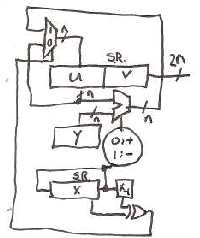
\includegraphics{booths.png}
\end{center}
\end{wrapfigure}

\textbf{Booth's Algorithm}
\begin{enumerate}
    \item group two regs (\emph{u},\emph{v}) for product, set to 0
    \item set \emph{$x_{-1}$} to 0 (this is a single bit)
    \item for each digit do:
    \begin{enumerate}
        \item if (lsb of \emph{x} is 1,) and (\emph{$x_{-1}$}=0), subtract \emph{y} from \emph{u}
        \item if (lsb of \emph{x} is 0) and (\emph{$x_{-1}$}=1), add \emph{y} to \emph{u}
        \item arithmetic right shift (\emph{u},\emph{v})
        \item circular right shift \emph{x}
    \end{enumerate}
\end{enumerate}

Booth's algorithm can be implemented in a circuit as is done in Figure~\ref{f-booths}.  Note the implementation is quite simple, only requiring shift registers, a mux, an adder (any type you like), and an xor.



\begin{example}
Multiply $6$ ($x=0110$) and $-1$ ($y=1111$) using Booth's algorithm.  Show the values at each stage in a table.

       {\color{ans}
       Booth's

       \begin{tabular}{cccc}
         $u$ & $v$ & $x$ & $x_{-1}$ \\ \hline
         0000 & 0000 & 1111 & 0 \\ \hline
         1010 & 0000 &   &   \\
         1101 & 0000 & 1111 & 1 \\ \hline
         1110 & 1000 & 1111 & 1 \\ \hline
         1111 & 0100 & 1111 & 1 \\ \hline
         1111 & 1010 & 1111 & 1 \\
       \end{tabular}

       Note the answer is 11111010, which is $-6$ in 2's complement.
       }
\end{example}

\begin{example}
Multiply -3 and 5 using Booth's algorithm and 4 bit numbers.  Perform the indicated calculations showing all steps.

    {\color{ans}
    $y=5=0101$

    $-y=-5=1011$

    \begin{tabular}{|c|c|cc|} \hline
      $u$  & $v$  & $x$  & $x_{-1}$ \\ \hline
      0000 & 0000 & 1101 & 0 \\ \hline
      1011 &      &      &   \\ \cline{1-1}
      1011 & 0000 & 1101 & 0 \\
      1101 & 1000 & 1110 & 1 \\ \hline
      0101 &      &      &   \\ \cline{1-1}
      0010 & 1000 & 1110 & 1 \\
      0001 & 0100 & 0111 & 0 \\ \hline
      1011 &      &      &   \\ \cline{1-1}
      1100 & 0100 & 0111 & 0 \\
      1110 & 0010 & 1011 & 1 \\ \hline
      1111 & 0001 & 1101 & 1 \\ \hline
    \end{tabular}

    The result is 11110001, which is $-15$ in 2's complement.
    }
\end{example}

\begin{example}
Multiply -3 and -6 using Booth's algorithm and 4 bit numbers.  Perform the indicated calculations showing all steps.

    {\color{ans}

    $x=-3=1101$, $y=-6=1010$ and $-y=6=0110$.

    \begin{tabular}{|c|c|c|c|}
      \hline
      $U$ & $V$ & $X$ & $X_{-1}$ \\ \hline
      0000 & 0000 & 1101 & 0 \\ \hline
      0110 & 0000 & 1101 & 0 \\
      0011 & 0000 & 1110 & 1 \\ \hline
      1101 & 0000 & 1110 & 1 \\
      1110 & 1000 & 0111 & 0 \\ \hline
      0100 & 1000 & 0111 & 0 \\
      0010 & 0100 & 1011 & 1 \\ \hline
      0001 & 0010 & 1101 & 1 \\ \hline
    \end{tabular}

    $00010010=18$
    }
\end{example}

